\documentclass{proc}

\usepackage[margin=1in]{geometry}
\usepackage{multirow}
\usepackage{arydshln}
\usepackage{graphicx}
\usepackage{caption, subcaption}

\title{More on Tables and Graphics}
\author{Javad M Alizadeh}
\date{}

\begin{document}
\maketitle
	
\section{Introduction}

Here we'll look at more table and graphics formatting.


\subsection{More on Tables}

Table~\ref{tab:wrapping} uses text wrapping in the last column.

\begin{table}[htbp]
	\caption{Text Wrapping}
	\begin{center}
		\begin{tabular}{|c|c|p{3cm}|}
			\hline
			CS101 & Java & Programming with Java \\
			CS201 & Languages & Programming language principles \\
			CS301 & Compilers & Principles of compiler design and implementation \\
			\hline
		\end{tabular}
	\end{center}
\label{tab:wrapping}	
\end{table}

Table~\ref{tab:multi} uses row and column span.

\begin{table}[htbp]
	\caption{Spanning rows and columns}
	\begin{center}
		\begin{tabular}{|c|c|c|}
			\hline
			& \multicolumn{2}{c|}{Ranges} \\
			\cline{2-3}
			& X & Y \\
			\hline
			\multirow{3}{*}{Hot} & 7 & 9 \\
			& 5 & 8 \\
			& 6 & 7 \\\hdashline 
			\multirow{3}{*}{Cold} & 7 & 9 \\
			& 5 & 8 \\
			& 6 & 7 \\
			\hline
		\end{tabular}
	\end{center}
	\label{tab:multi}	
\end{table}
	

\subsection{More on graphics}

Both of my graphics are in the graphics folder for the subfigures, Figure~\ref{fig:paper} and Figure~{fig:page} in Figure~\ref{fig:subs}.

\begin{figure}
\centering
	\begin{subfigure}[b]{0.2\textwidth}
		\centering
		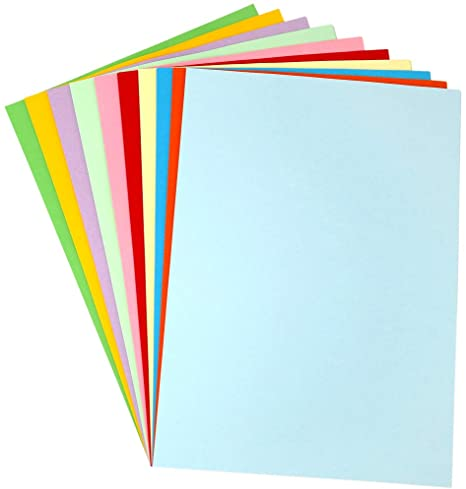
\includegraphics[scale=0.2]{paper.jpg}
		\caption{Beginning}
		\label{fig:paper}
	\end{subfigure}
	\begin{subfigure}[b]{0.2\textwidth}
		\centering
		
\includegraphics[scale=0.03]{page.jpeg}
		\caption{End}
		\label{fig:page}
	\end{subfigure}
\caption{The process}
\label{fig:subs}
\end{figure}
	
	
\section{Conclusion}
	
	
\end{document}
